\documentclass[10pt]{beamer}
\usepackage{graphicx}
\usepackage{amsmath}
\usepackage{bibentry}
\usepackage{biblatex}
\usepackage{adjustbox}
\usepackage[font=scriptsize]{caption}
\usepackage{subcaption}
\usepackage{hyperref}
\captionsetup[figure]{labelsep=period}
\captionsetup[subfigure]{labelformat=simple} % default is 'parens'
\renewcommand\thesubfigure{\thefigure.\alph{subfigure}.}
\DeclareMathOperator*{\argmax}{argmax}
\DeclareMathOperator*{\argmin}{argmin}

\setbeamertemplate{navigation symbols}{}
\setbeamertemplate{caption}[numbered]
\bibliography{Bibliography}

\graphicspath{{images/}}
\setbeamertemplate{footline}[frame number]
\setbeamertemplate{page number in head/foot}[appendixframenumber]
\usetheme{Darmstadt}

\title[short]{INTELLIGENT SYSTEMS}
\author[Flavio Forenza]{Flavio Forenza \\ \tiny flavio.forenza@studenti.unimi.it\\[5mm] 
\includegraphics[scale = 0.06]{logoUnimi2.png}}
\institute{Department of Computer Science,\\ University of Milan, Italy}
\date{\tiny \today}

\begin{document}

\begin{frame}
    \maketitle
\end{frame}


\logo{
\includegraphics[width=0.1\linewidth]{logoUnimi2.png}}
\section{Paper 1}
\subsection{\emph{"A Unified Framework for Salient StructureDetection by Contour-Guided Visual Search"}}
\begin{frame}{INTRODUCTION}
    The purpose of the paper is to introduce a new method, called CGVS in the 
    state of the art, which is able to identify regions and salient objects 
    within a scene simultaneously. The proposed system attempts to 
    bridge the gap between the two highly related tasks of \emph{"human 
    fixation"} prediction and \emph{"salient object detection"}, with a general 
    framework.
\end{frame}

\begin{frame}{RELATED WORK}
    To obtain the final result, two pathways are crossed (Fig.\ref{fid: flowchart}):
    \begin{enumerate}
        \item Selective
        \item Non-Selective
    \end{enumerate}
    \begin{figure}[htbp]
        \centering
        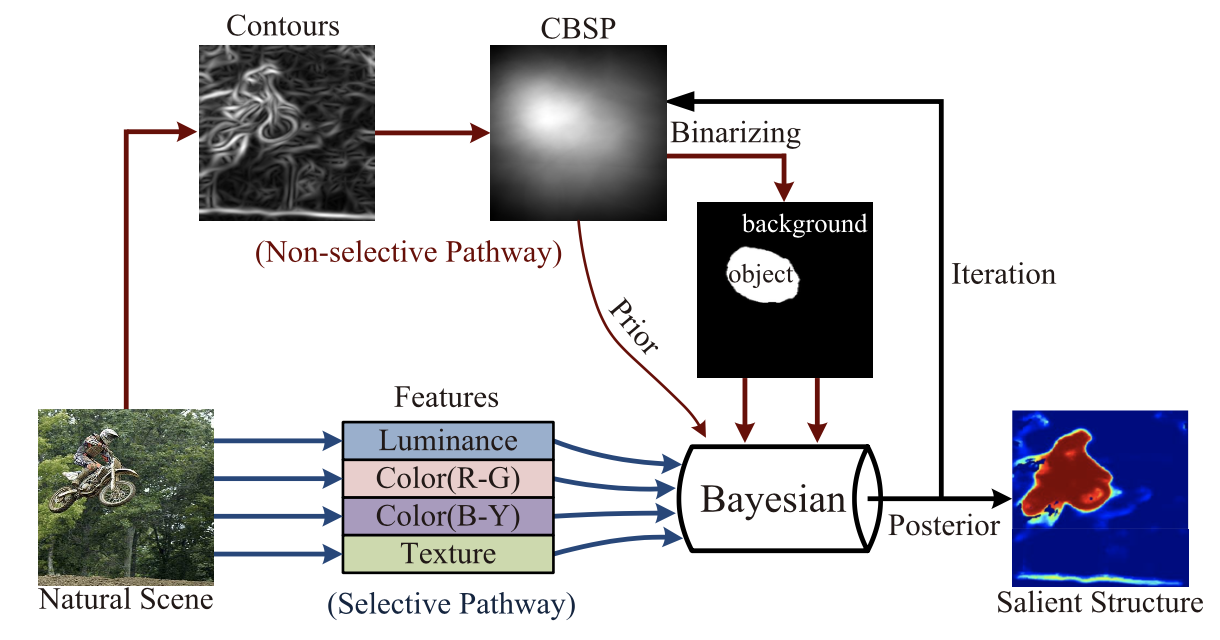
\includegraphics[width = 0.8\linewidth]{images/paper1/selective and non-selective pathways.png}
        \centering
        \caption{The flowchart of the porposed system.}
        \label{fid: flowchart}
    \end{figure}
\end{frame}

\begin{frame}[t]{CONTOUR-GUIDED VISUAL SEARCH MODEL pt1}
    In \emph{Non-Selective} pathway are computed:
    \begin{enumerate}
        \item \emph{Boundary} \footfullcite{0747815570}
        \item \emph{Contour-Based Spatial Prior (CBSP)} $ \rightarrow S_w = S_e + S_c $
    \end{enumerate}
    \begin{figure}[htbp]
        \centering
        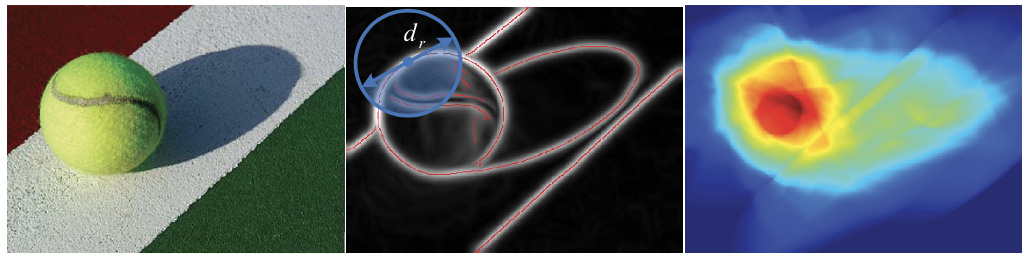
\includegraphics[width = 0.5\linewidth]{images/paper1/CBSP.png}
        \centering
        \caption{CBSP reconstruction.}\vspace{0mm}
        \label{fid: CBSP}
    \end{figure}
    In \emph{Selective} pathway are computed the basic low-level features:
    \begin{enumerate}
        \item \emph{Luminance} $ \rightarrow f_{lum} = (r+g+b)/3 $
        \item \emph{Color-Opponent} $ \rightarrow f_{rg} = r-g , f_{by} = b-(r+g)/2 $
        \item \emph{Texture Channel} ($ f_{ed} $)
    \end{enumerate}
\end{frame}

\begin{frame}[t]{CONTOUR-GUIDED VISUAL SEARCH MODEL pt2}
    \begin{block}{Bayesian inference}
        All the previous informations are used to compute the Bayesian inference:
        $$ p(s|x) = \frac{p(s)p(x|s)}{p(s)p(x|s)+p(b)p(x|b) } $$
    \end{block}
    Where:
    \begin{enumerate}
        \item $ p(x|s) \rightarrow $ likelihood of a pixel at \emph{x} belonging to a salient structure \emph{s}
        \item $ p(x|b) \rightarrow $ likelihood of a pixel at \emph{x} belonging to the background \emph{b}
        \item $ p(s) \mbox{ and } p(b)=1-p(s) \rightarrow $ prior probabilities of a pixel at x belonging to a salient structure and the background, respectively.
    \end{enumerate}
\end{frame}

\begin{frame}{CONTOUR-GUIDED VISUAL SEARCH MODEL pt3}
    To compute the prior probabilities, we need:
    \begin{enumerate}
        \item \emph{Predict the Size of Potential Structure}: using a optimal threshold ($ T_{opt} $) 
        useful for separating the background from the foreground (salient structures).
        \item \emph{Evaluate the Importance of Each Feature}: weighing every salient structure.
        \item \emph{Calculate the Observation Likelihood:} both $ p(x|s) \mbox{ and } p(x|b) $
        \item \emph{Enhance the Salient Structure by Iterating}: we re-initialize the prior 
        function with the smoothed version of $ p(s|x) $ (by median filtering 
        with a size of 21 × 21 pixels)
    \end{enumerate}
\end{frame}

\begin{frame}[t]{EXPERIMENTS}
    The results obtained on different datasets \footfullcite{PASCAL-S, ECSSD, ASD}, were compared with those 
    btained by the systems already existing at the state of the art.
    \begin{figure}[htbp]
        \centering
        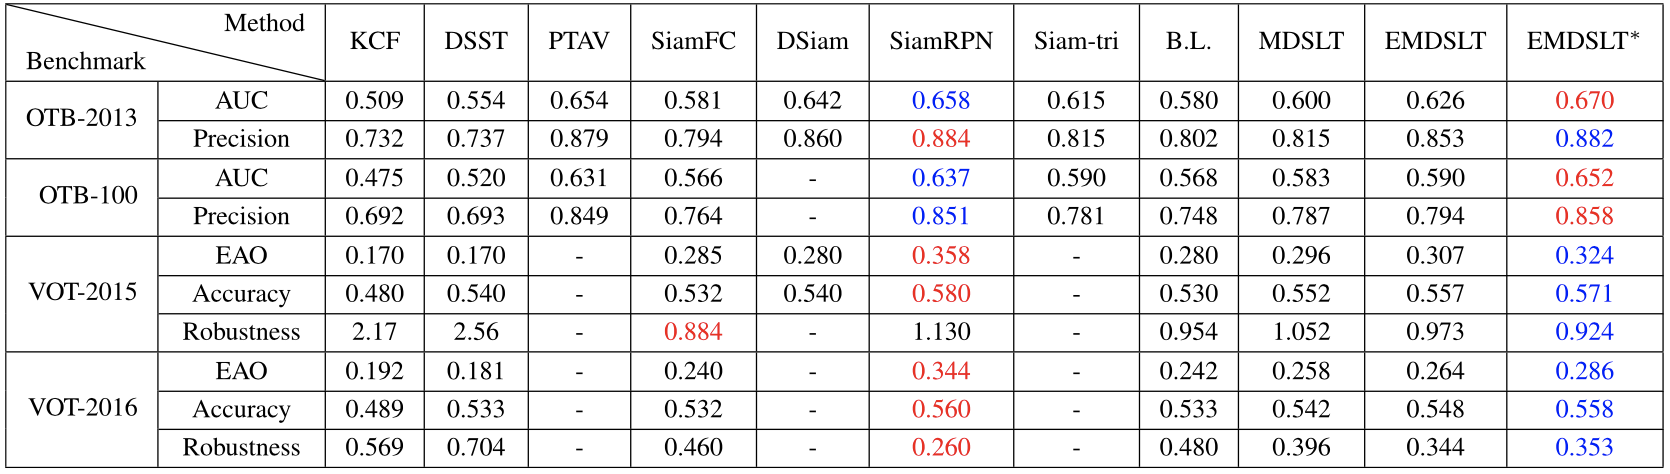
\includegraphics[width = 0.8 \linewidth]{/paper1/metrics.png}
        \centering
        \caption{Metrics comparison.}
        \label{fig: metrics}
    \end{figure}
\end{frame}

\begin{frame}{DISCUSSION}
    It is necessary to say that the results obtained by the proposed method 
    are obtained using the center bias, which if removed places the system 
    performance under those of systems such as \emph{RF} \footfullcite{0747815518} and \emph{HS}\footfullcite{0747815508} (which do not 
    use the central bias). This method offers a dual use. In 
    a cluttered scene with no dominant objects, the system will function as a 
    fixation prediction model. Finally, on the other hand, with simple scenes, 
    the system detects existing relevant objects.
    \begin{figure}[htbp]
        \centering
        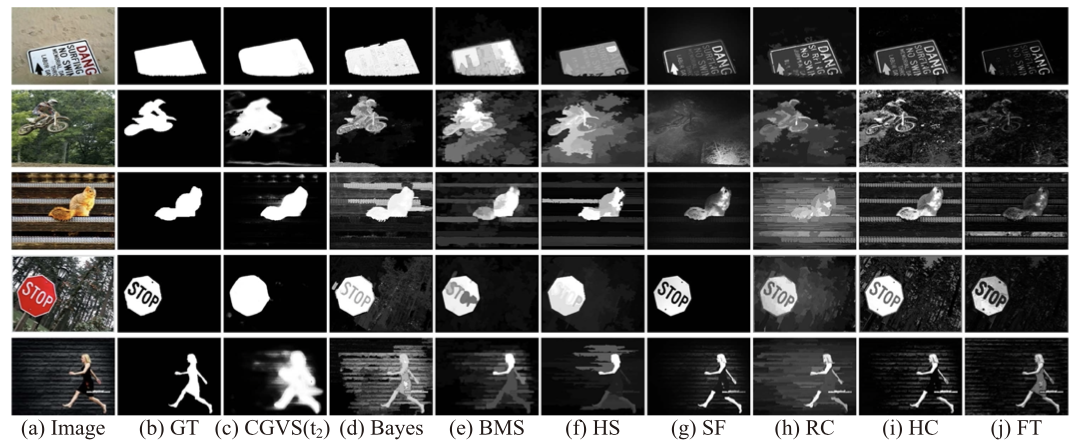
\includegraphics[width = 0.7 \linewidth]{paper1/SystemsComp.png}
        \centering
        \label{fig: metrics}
    \end{figure}
\end{frame}

\section{Paper 2}
\subsection{\emph{"Linear Spectral Clustering Superpixel"}}
\begin{frame}{INTRODUCTION}
    The introduced technique is called SUPERPIXEL. Widely used in image 
    processing for particular tasks such as image segmentation, image analysis, 
    image classification, target tracking, 3D reconstruction, surface retrieval and 
    object proposal. The purpose of the elaborate story is to reduce the 
    computational complexity through a superpixel system called LSC (Linear Spectral
    Clustering).
\end{frame}

\begin{frame}{LSC SUPERPIXEL pt1}
    Goal: optimization (max/min) of two objective functions to create clusters of pixels called superpixels:
    \begin{block}{Objective Function 1: Weighted K-Means}
        $$ F_{km} = \sum_{k=1}^K\sum_{p\in\pi_k}\omega(p)= || \phi(p)-m_k ||^2 $$
    \end{block}
    \begin{block}{Objective Function 2: Normalized cuts}
        $$ F_{N_{cuts}} = \frac{1}{K}\sum_{k=1}^K\frac{\sum_{p\in\pi_k}\sum_{q\in\pi_k}W(p,q)}{\sum_{p\in\pi_k}\sum_{q\in{V}}W(p,q)} $$
    \end{block}
    Problem: extremely high computational!
\end{frame}

\begin{frame}{LSC SUPERPIXEL pt2}
    If corollary 1 is satisfied, then  \emph{weghted K-means clustering} can be used 
    for segmentation and for creation of superpixel regions, instead of the 
    eigen-vector based method.
    \begin{block}{\bfseries{Corollary 1}}
        Optimizations of the objective functions of the weighted K-means
        and the normalized cuts are mathematically equivalent if (1) and (2) 
        hold simultaneously. The symbol $ \cdot $ stands for inner product.
    \end{block}

    \begin{block}{Equation (1)}
           $$ \omega(p)\phi(p) \cdot \omega(q)\phi(q) = W(p,q), \forall p,q \in V $$
    \end{block}

    \begin{block}{Equation (2)}
        $$ \omega(p) = \sum_{q \in V} W(p,q), \forall p \in V $$
    \end{block}
\end{frame}

\begin{frame}{LSC Algorithm pt1}
    Problem? $ \rightarrow $ Find the correct positive similarity function $ W (p,q) $, 
    between two data points \emph{p} and \emph{q} to solve equation 1.
    \begin{block}{Similarity Function}
        \begin{equation}\small
            \begin{split}
                W(p,q) = C_s^2(\cos \frac{\pi}{2}(x_p-x_q)+\cos\frac{\pi}{2}(y_p-y_q)) \\
                + C_c^2(\cos \frac{\pi}{2}(l_p-l_q)+\cos\frac{\pi}{2}(\alpha_p-\alpha_q) \\
                + \cos\frac{\pi}{2}(\beta_p-\beta_q)x2.55^2)
            \end{split}
        \end{equation}
    \end{block}
    
    \begin{block}{Mapping Function}
        \begin{equation}\small
            \begin{split}
                \phi(p) = \frac{1}{\omega(p)}[C_c\cos\frac{\pi}{2}l_p, C_c\sin\frac{\pi}{2}l_p, 2.55C_c\cos\frac{\pi}{2}\alpha_p \\
                x 2.55C_c\sin\frac{\pi}{2}\alpha_p, 2.55C_c\cos\frac{\pi}{2}\beta_p, 2.55C_c\sin\frac{\pi}{2}\alpha_p, \\
                x C_s\cos\frac{\pi}{2}x_p, C_s\sin\frac{\pi}{2}x_p, C_s\cos\frac{\pi}{2}y_p, C_s\sin\frac{\pi}{2}x_p]
            \end{split}
        \end{equation} 
    \end{block}
    
\end{frame}

\begin{frame}{LSC Algorithm pt2}
    Assuming that equation 1 exists, LSC method takes two parameters as 
    input; The image to be segmented and the preferred K number of 
    superpixels that the algorithm will have to produce. The number K 
    corresponds to the number of centroids and each of these will be useful 
    for grouping the neighbors pixels, in a range of $ \tau v_x \ x \ \tau v_y $, with $ \tau>0.5 $, 
    using a distance comparison.
    \begin{figure}[h!]
        \centering
        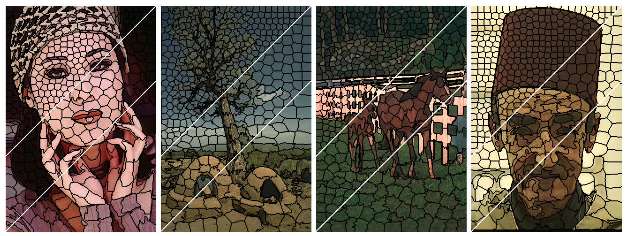
\includegraphics[width = 0.7 \linewidth]{paper2/slide1.png}
        \centering
        \caption{Sample images segmented with K = 1000/500/200 superpixels using LSC.}
        \label{fig: metrics}
    \end{figure}
\end{frame}

\begin{frame}{COMPARATIVE EXPERIMENTS}
    \begin{table}[htbp!]
        \centering
        \begin{adjustbox}{max width=\textwidth}
        \begin{tabular}{*{9}{|c}|}%%{|c|c|c|c|c|c|c|c|c|}
            \hline
            & EneOpt0 & SEEDS\footfullcite{0781426509} & ERS\footfullcite{0781426508} & Lattices & NCuts & SLIC\footfullcite{0781426514} & Turbo & LSC \\
            \hline
            \bfseries{ADERENCE TO BOUNDARY} & & & & & & & & \\
            \emph{Under segmentation error} & 0.230 & 0.197 & 0.198 & 0.303 & 0.220 & 0.213 & 0.277 & \bfseries{0.190}\\
            \emph{Boundary recall} & 0.765 & 0.918 & 0.920 & 0.811 & 0.789 & 0.837 & 0.739 & \bfseries{0.926}\\
            \emph{Achievable segmentation accuracy} & 0.950 & 0.960 & 0.959 & 0.933 & 0.956 & 0.956 & 0.943 & \bfseries{0.962}\\
            \hline
            \bfseries{SEGMENTATION SPEED} & & & & & & & & \\
            \emph{Computational complexity} & $ O(N^3/K^2) $ & $ O(N) $ & $ O(N^2 \lg{N}) $ & $ O(N^{\frac{3}{2}} \lg{N}) $ & $ O(N^{\frac{3}{2}}) $ & $ O(N) $ & $ O(N) $ & $ O(N) $\\
            \emph{Average time per image} & 3.35s & \bfseries{0.0935}s & 0.969s & 0.284s & 93.4s & 0.125s & 6.61s & 0.334s\\
            \hline
        \end{tabular}
        \end{adjustbox}
        \caption{Performance metrics superpixel segmentation algorithms at K=400}
        \label{table superpixels}
    \end{table}
    Best performance: low "Under segmentation Error" (\emph{UE}), high 
    "Boundary Recall" (\emph{BR}) and high "Achievable segmentation accuracy 
    (\emph{ASA}).
\end{frame}

\begin{frame}{APPLICATIONS: Class segmentation}
    \begin{figure}[htbp]
        \centering
        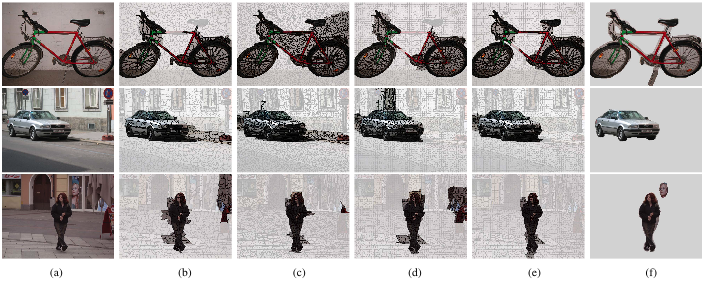
\includegraphics[width = 1 \linewidth]{images/paper2/superpixelAlgo.png}
        \centering
        \caption{Segmentation using different superpixels algorithms. (a) Original Image. (b) QS. (c) ERS. (d) SLIC. (e) LSC. (f)Ground Truth.}
        \label{fig: superpixelSegmentation}
    \end{figure}

    \begin{table}[h!]
        \centering
        \begin{adjustbox}{max width=4cm}
        \begin{tabular}{*{5}{|c}|}%%{|c|c|c|c|c|}
            \hline
            & QS & ERS & SLIC & LSC\\
            \hline
            bike & 72.2 & 74.2 & 76.3 & \bfseries{76.9}\\
            cars & 72.2 & 74.7 & 72.5 & \bfseries{76.8}\\
            person & 66.3 & 66.5 & 66.7 & \bfseries{67.0}\\
            \hline
        \end{tabular}
        \end{adjustbox}
        \caption{Accuracy using different superpixels algorithms.}
        \label{table accuracy}
    \end{table}
\end{frame}

\begin{frame}{APPLICATIONS: Weakly Supervised Semantic Segmentation}
    \begin{minipage}{\linewidth}
        \centering
        \begin{minipage}{0.45\linewidth}
            \begin{figure}[H]
                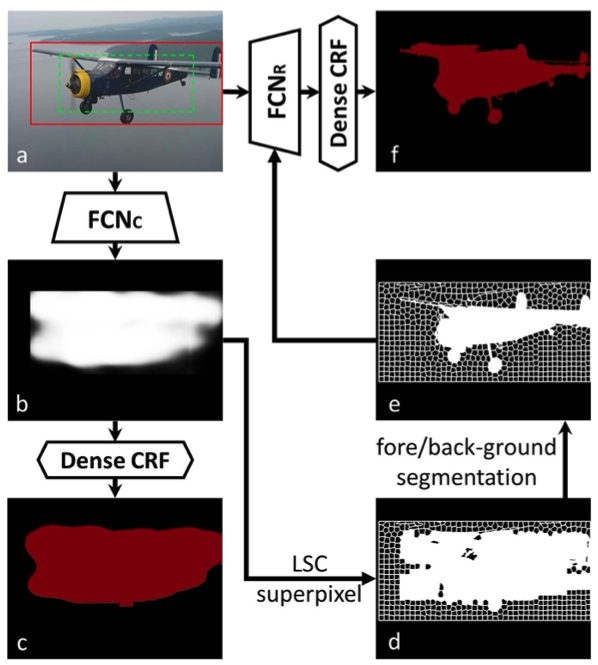
\includegraphics[width = 0.7 \linewidth]{images/paper2/semanticSegmentation.png}
                \caption{Weakly supervised semantic segmentation. (a) A training image with bounding boxes. (b) Output of soft-max layer of $ FCN_c $. (c) Coarse semantic segmentation result. (d) Superpixels with higher probability of foreground. (e) Fore-/Background segmentation result after iterative optimization. (f) Refined semantic segmentation result.}
            \end{figure}
        \end{minipage}
        \hspace{0.05\linewidth}
        \begin{minipage}{0.45\linewidth}
            \begin{figure}[htbp]
                \centering
                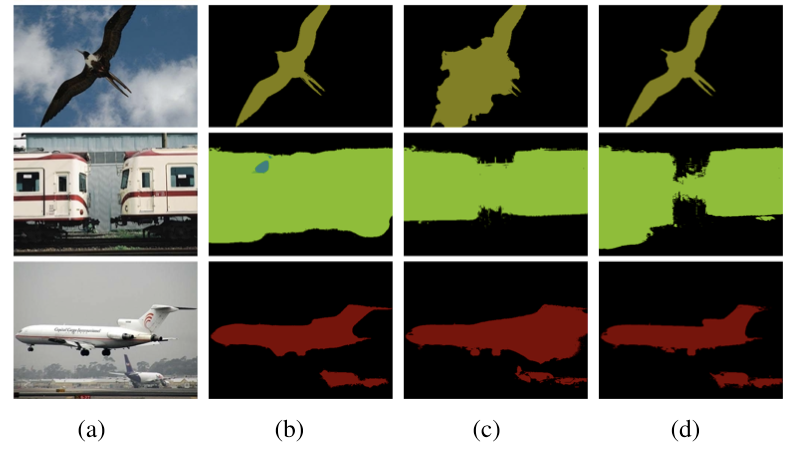
\includegraphics[width = 1 \linewidth]{images/paper2/segmentationAlgo.png}
                \centering
                \caption{Semantic segmentation. (a) Input image. (b) Strong. (c) Bbox-seg. (d) $ Joint_{sp} $ (LSC) }
            \end{figure}
            \begin{table}[H]
                \begin{adjustbox}{max width=4cm}
                    \begin{tabular}{*{3}{|c}|}%%{|c|c|c|}
                        \hline
                        Strong\footnotemark[1]& Bbox-seg\footnotemark[1] & $ Joint_{sp} $ \\
                        \hline
                        62.5 & 60.6 & \bfseries{64.0} \\
                        \hline
                    \end{tabular}
                \end{adjustbox}
                \caption{Semantic segmentation accuracy in terms of Mean IOU (\%)}
            \end{table}
        \end{minipage}
    \end{minipage}
    \footnotetext[1]{\tiny G. Papandreou, L. Chen, K. Murphy, and A. Yuille, “Weakly-and semi-
    supervised learning of a deep convolutional network for semantic image segmentation,” in Proc. ICCV, pp. 1742–1750, Dec. 2015}
\end{frame}

\begin{frame}{CONCLUSIONS}
    The LSC algorithm seems to be the best in terms of adherence to the 
    boundary and in the creation of superpixels with increasingly regular 
    shape, but there are still two problems to solve:
    \begin{enumerate}
        \item The number K of superpixels entered manually
        \item New similarity techniques to improve performance
    \end{enumerate}
\end{frame}

\section{Paper 3}
\subsection{\emph{"An End-to-End Compression Framework Based on Convolutional Neural Networks"}}

\begin{frame}{INTRODUCTION}
    In recent years, within the field of computer vision, remarkable results 
    have been achieved with regard to image compression. The purpose of 
    compressionis to be able to transmit, or save, the entire image at low bit 
    rates. The following article presents a compression method based on 
    convolutional neural networks (CNNs) which, through the use of various 
    state-of-the-art codecs, are able to achieve better performance in terms 
    of compression and image quality.
\end{frame}

\begin{frame}{RELATED WORK}
    At the state of the art there are post-processing methods that use 
    {\bfseries{deblocking}} and {\bfseries{restoring}} techniques \footfullcite{0799924108}. These techniques have a strong 
    computational impact on systems. These operations focus on eliminating 
    artifacts and blocks that contain noise within the image. Other methods 
    use CNNs for {\bfseries{super-resolution}} (SR) images \footfullcite{0799924123}. There are deep learning 
    methods that are used for {\bfseries{lossy}} \footfullcite{0799924125} or {\bfseries{lossless}} \footfullcite{0799924130} compression of images, but 
    these ignore the use of the various existing codecs.
\end{frame}

\begin{frame}{THE PROPOSED COMPRESSION FRAMEWORK pt1}
    The proposed system is composed of two convolutional neural networks:
    \begin{enumerate}
        \item \emph{ComCNN}: used for compact representation of images
        \item \emph{RecCNN}: used for decoding and reconstruction of images
    \end{enumerate}
    \begin{figure}[htbp]
        \centering
        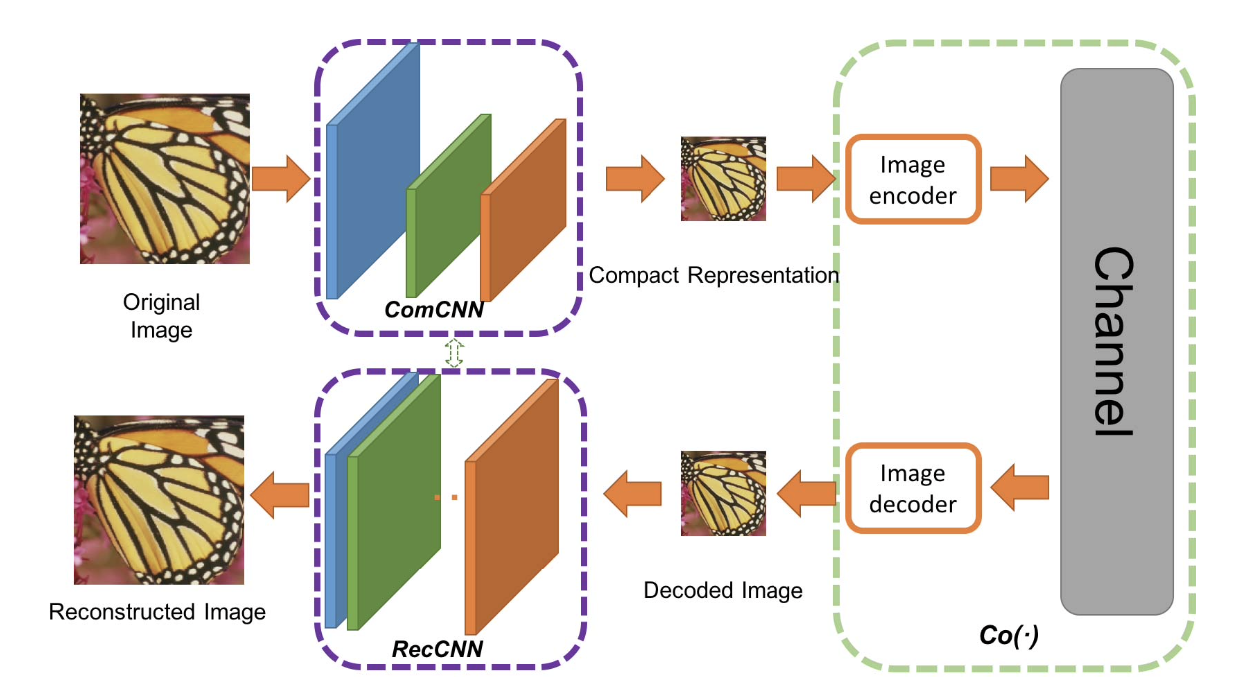
\includegraphics[width = 0.8 \linewidth]{images/paper3/framework.png}
        \centering
        \caption{Up: the ComCNN. Down: the RecCNN. Right: the codec.}
        \label{fig: framework}
    \end{figure}
\end{frame}

\begin{frame}{THE PROPOSED COMPRESSION FRAMEWORK pt2}
    \begin{minipage}{\linewidth}
        \centering
        \begin{minipage}{0.45\linewidth}
            \begin{figure}[H]
                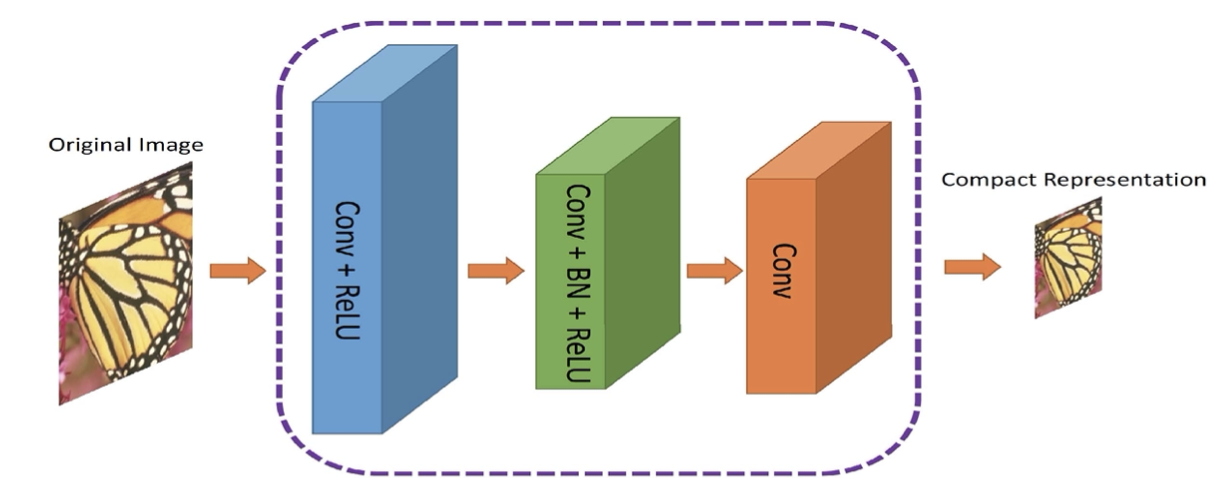
\includegraphics[width = 1 \linewidth]{images/paper3/ComCNN.png}
                \caption{ComCNN architecture.}
            \end{figure}
            \begin{block}{Parameter optimizations}
                \small $$ \hat{\theta_1} = \argmin\limits_{\theta_1}||Re(\hat{\theta_2},Cr(\theta_1,x))-x||^2 $$
            \end{block}
            \begin{block}{Loss Function}
               \tiny $$ L_1(\theta_1) = \frac{1}{2N}\sum_{k=1}^N||Re(\hat{\theta_2}, C_r(\theta1,x_k))-x_k||^2 $$
            \end{block}
        \end{minipage}
        \hspace{0.05\linewidth}
        \begin{minipage}{0.45\linewidth}
            \begin{figure}[htbp]
                \centering
                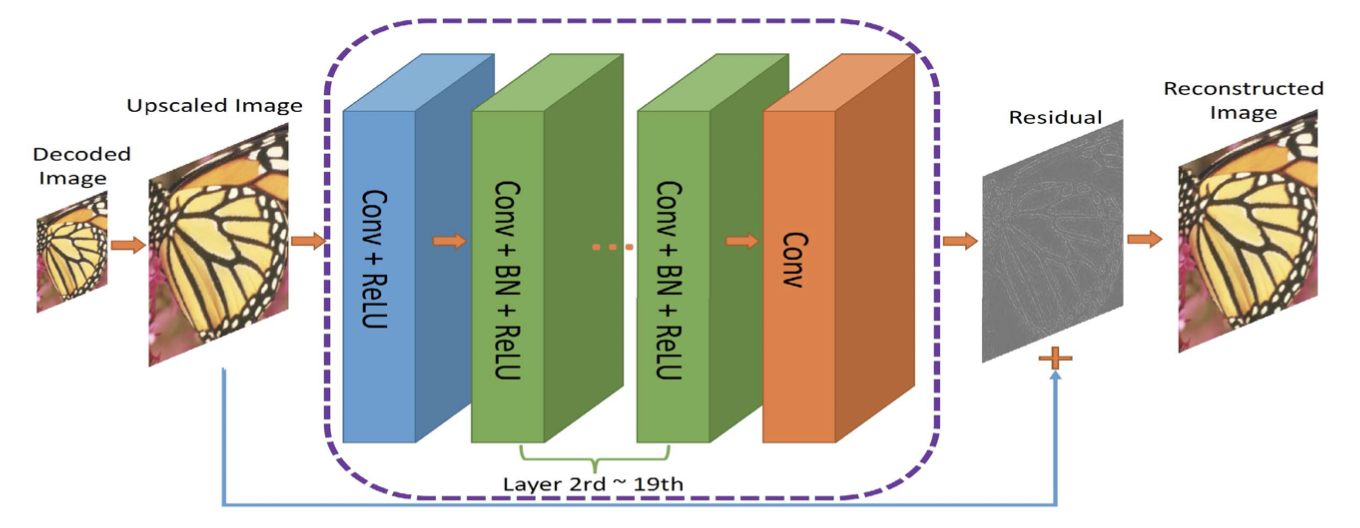
\includegraphics[width = 1 \linewidth]{images/paper3/RecCNN.png}
                \centering
                \caption{RecCNN architecture.}
            \end{figure}
            \begin{block}{Parameter optimizations}
                \small $$ \hat{\theta_2} = \argmin\limits_{\theta_2}||Re(\hat{\theta_2},\hat{x}_m)-x||^2 $$
            \end{block}
            \begin{block}{Loss Function}
                \tiny $$ L_2(\theta_2) = \frac{1}{2N}\sum_{k=1}^N||res(Co(\hat{x}_{mk}), \theta_2) - (Co(\hat{x}_{mk})-x_k)||^2 $$
             \end{block}
        \end{minipage}
    \end{minipage}
\end{frame}

\begin{frame}{EXPERIMENTS}
    The performance comparison is made by citing various techniques present 
    at the state of the art. A compression quality index ({\bfseries\emph{PSNR}}) and ù
    an image similarity index ({\bfseries\emph{SSIM}}) are used. What is really important to note 
    is how the proposed method manages to have better performance than 
    the already used codecs such as \emph{JPEG}, \emph{JPEG2000} and \emph{BPG}, at different 
    bit rates (\emph{bpp}) and quality factors (\emph{QS}). As for the execution times, in 
    terms of CPU / GPU, the proposed algorithm is faster than those already 
    existing.
    \begin{figure}[htbp]
        \centering
        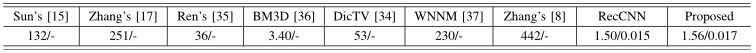
\includegraphics[width = 1 \linewidth]{images/paper3/time.png}
        \centering
        \caption{Running time(s) of compared methods in CPU (/GPU) }
        \label{fig:time}
    \end{figure}
\end{frame}

\begin{frame}{EXPERIMENTS: JPEG vs. The proposed system}
    With a variable QF (first set to 5 and then to 10), the results obtained by 
    the various methods, in terms of PSNR and SSIM, are shown in the following figures:
    \begin{minipage}{\linewidth}
        \centering
        \begin{minipage}{0.45\linewidth}
            \begin{figure}[H]
                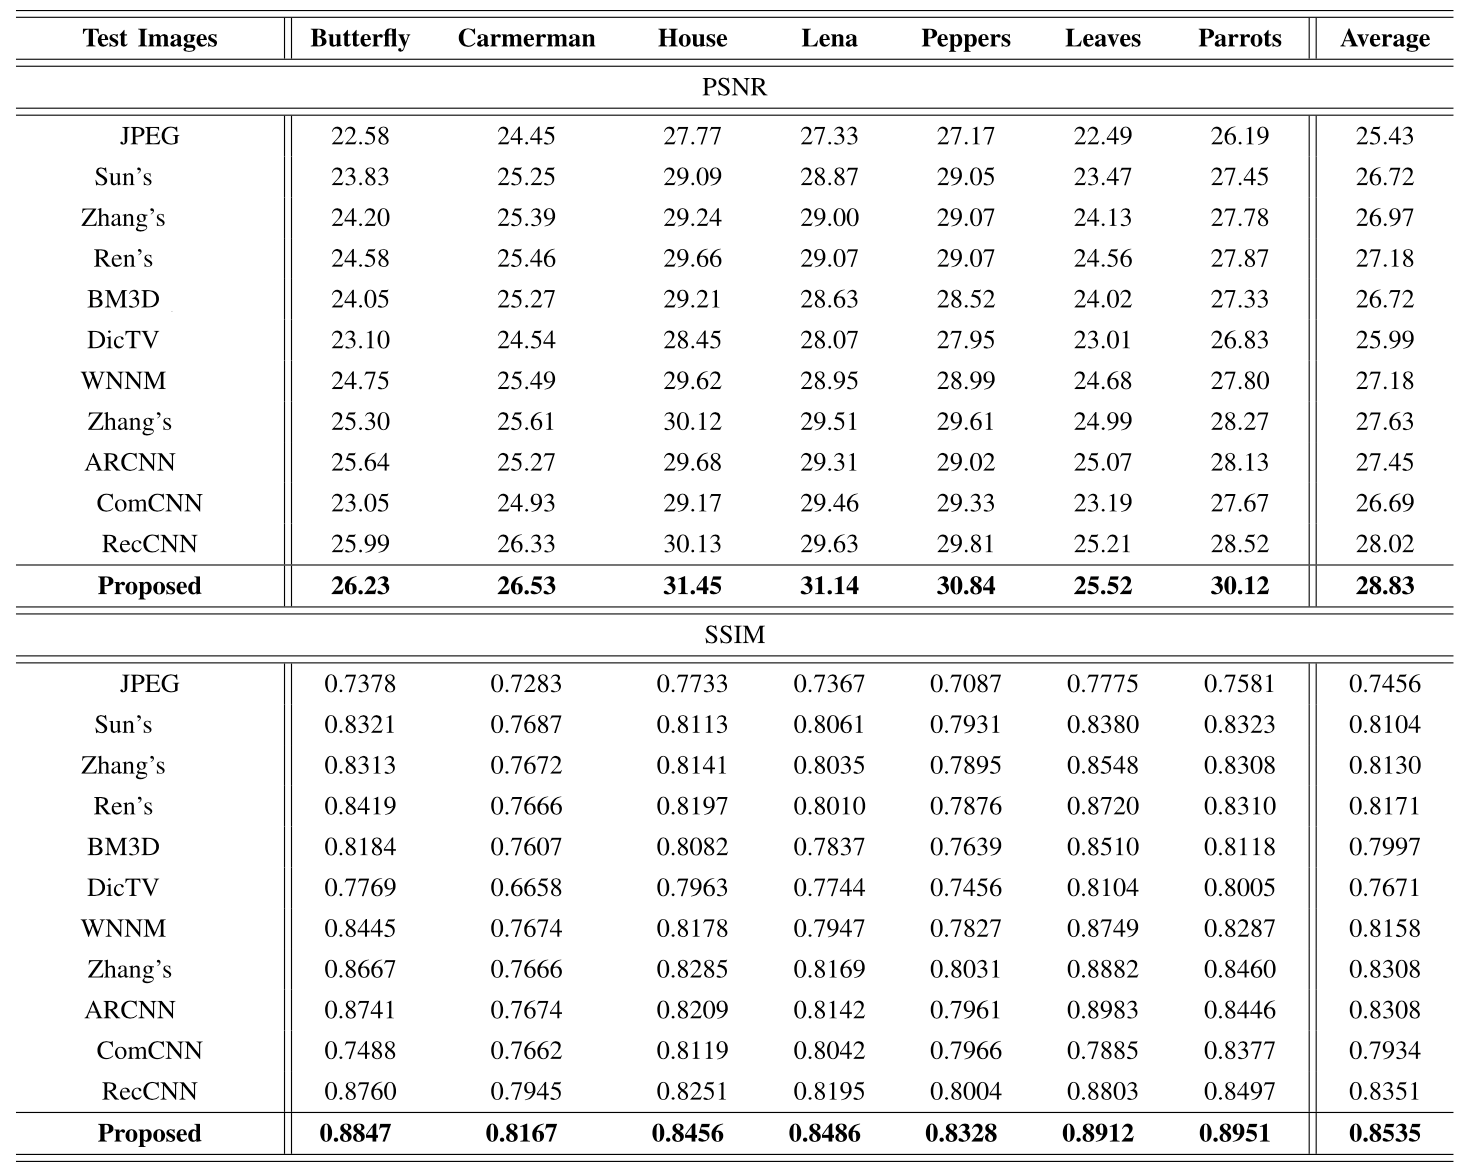
\includegraphics[width = 1 \linewidth]{images/paper3/comparison.png}
                \caption{QF = 5, PSNR(db) and SSIM results of alghoritms image deblocking and denoising}
            \end{figure}
        \end{minipage}
        \hspace{0.05\linewidth}
        \begin{minipage}{0.45\linewidth}
            \begin{figure}[htbp]
                \centering
                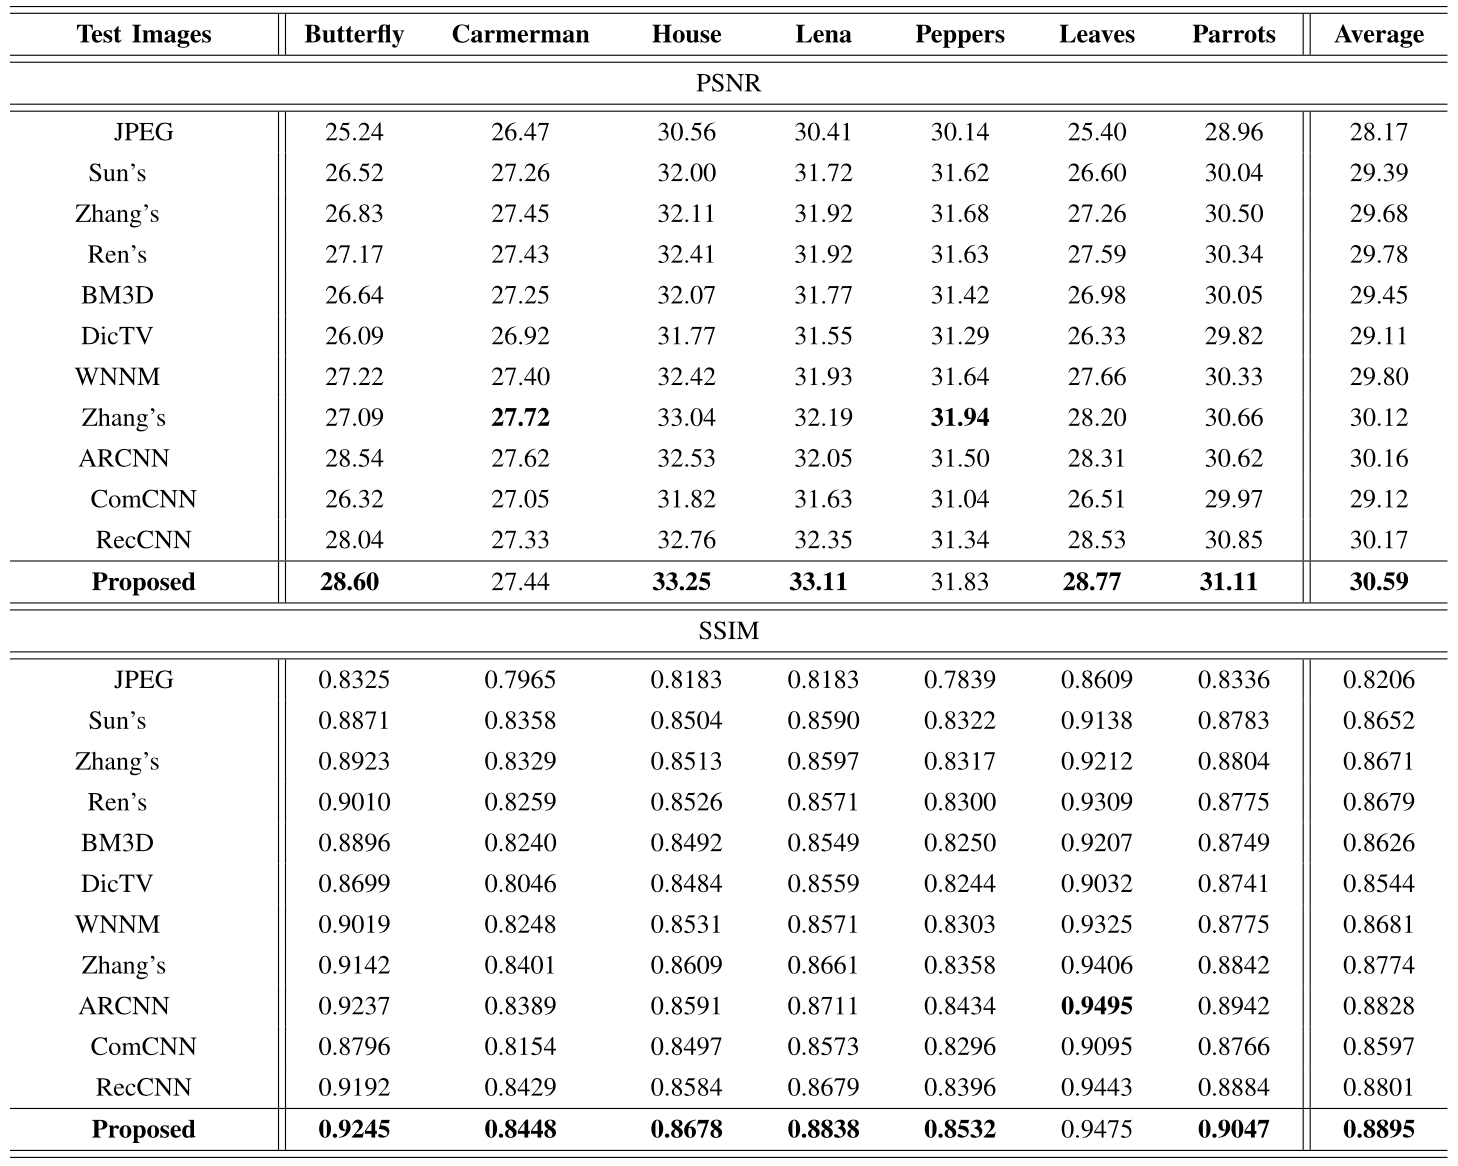
\includegraphics[width = 1 \linewidth]{images/paper3/comparison2.png}
                \caption{QF = 10, PSNR(db) and SSIM results of alghoritms image deblocking and denoising}
                \centering
            \end{figure}
        \end{minipage}
    \end{minipage}
\end{frame}

\begin{frame}{EXPERIMENTS: JPEG2000 vs. The proposed system}
    As we can see from the comparison made in figure \ref{fig:parrot}, the difference in  
    visual quality between the proposed method and the JPEG2000 codec is 
    considerable. With the same amount of bit rates, the JPEG2000 codec 
    produces worse results by losing several structural information. 
    \begin{minipage}{\linewidth}
        \centering
        \begin{minipage}{0.45\linewidth}
            \begin{figure}[H]
                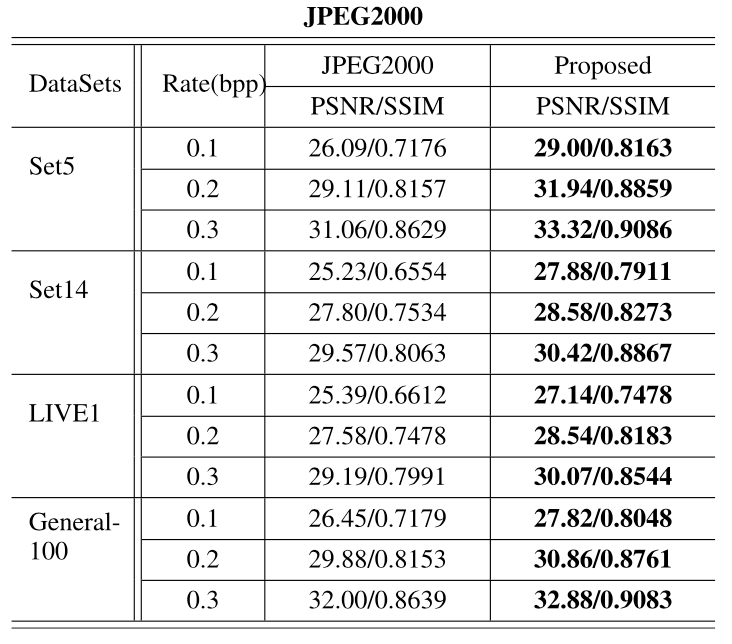
\includegraphics[width = 1 \linewidth]{images/paper3/JPEG2000.png}                
                \caption{Average PSNR(dB)/SSIM results of JPEG2000 and the proposed method on different datasets.}
            \end{figure}
        \end{minipage}
        \hspace{0.05\linewidth}
        \begin{minipage}{0.45\linewidth}
            \begin{figure}[htbp]
                \centering
                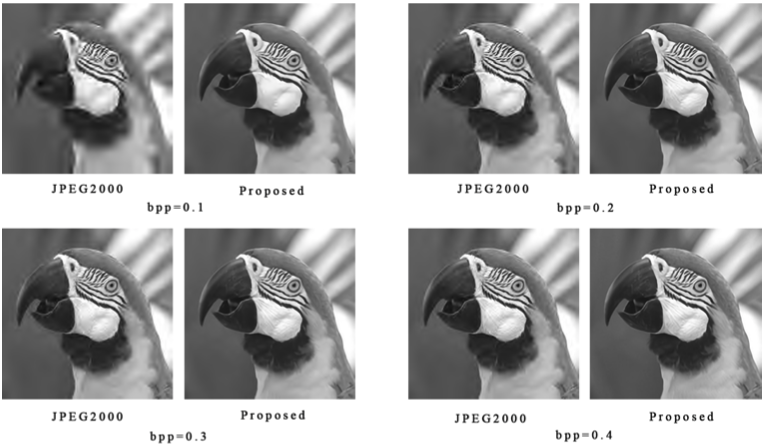
\includegraphics[width = 1 \linewidth]{images/paper3/JPEG2000p.png}
                \caption{Performance comparison of JPEG2000 at difference bit rates.}
                \label{fig:parrot}
                \centering
            \end{figure}
        \end{minipage}
    \end{minipage}
\end{frame}

\begin{frame}{EXPERIMENTS: BPG vs. The proposed system}
    As for the BPG codec, if used in combination with the \emph{ComCNN} and 
    \emph{RecCNN} networks, it reaches higher \emph{PSNR} and \emph{SSIM} levels than when 
    used individually or with only one of the two networks.   
    \begin{figure}[htbp]
        \centering
        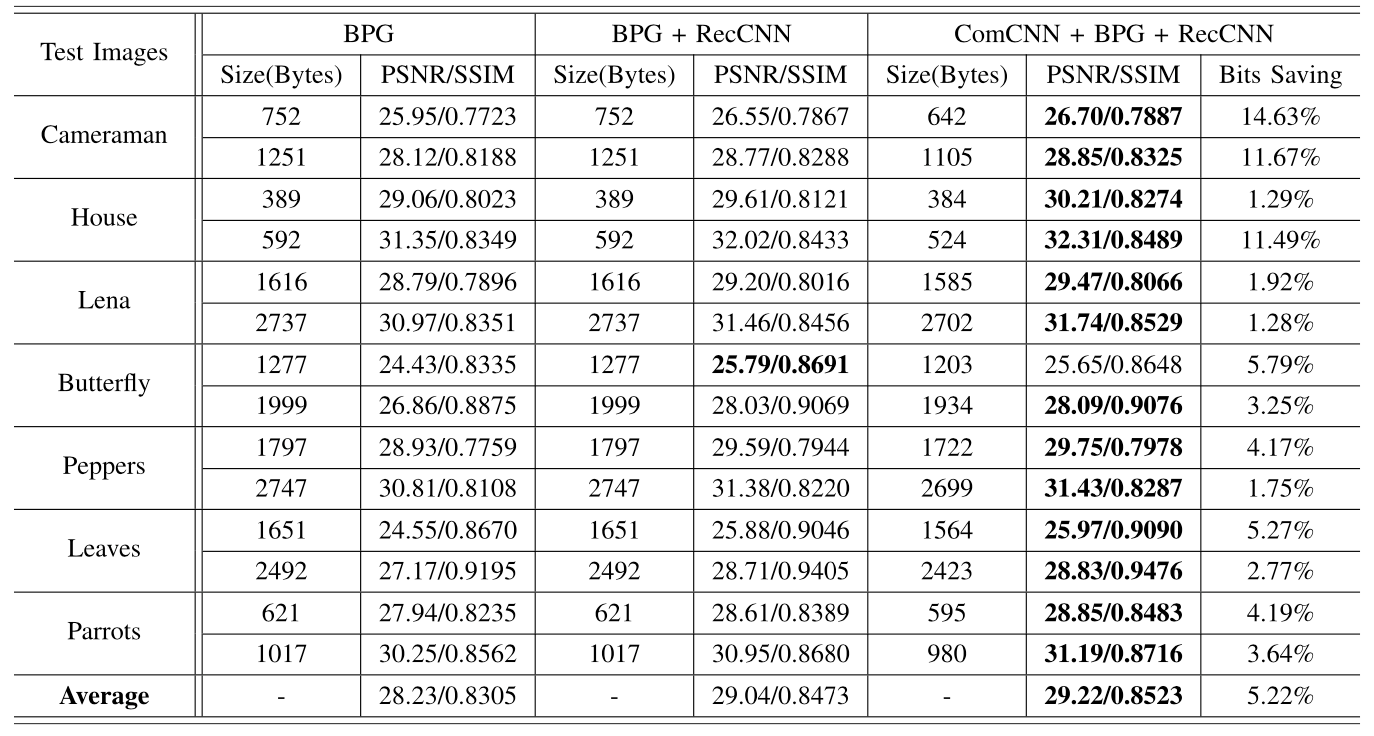
\includegraphics[width = 1 \linewidth]{images/paper3/BPG.png}
        \centering
        \caption{BPG: PSNR (dB) and SSIM result of BPG, BPG + RecCNN and the proposed method.}
        \label{fig:BPG}
    \end{figure}
\end{frame}

\begin{frame}{CONCLUSION}
    The proposed method seems to have the best performance compared to other 
    methods already existing in the state of the art. The proposed technique 
    then validates the use of one or more convolutional neural networks to carry 
    out the task of encoding and decoding images, even in some cases achieving 
    better quality than existing codecs for image compression.
    \begin{figure}[htbp]
        \centering
        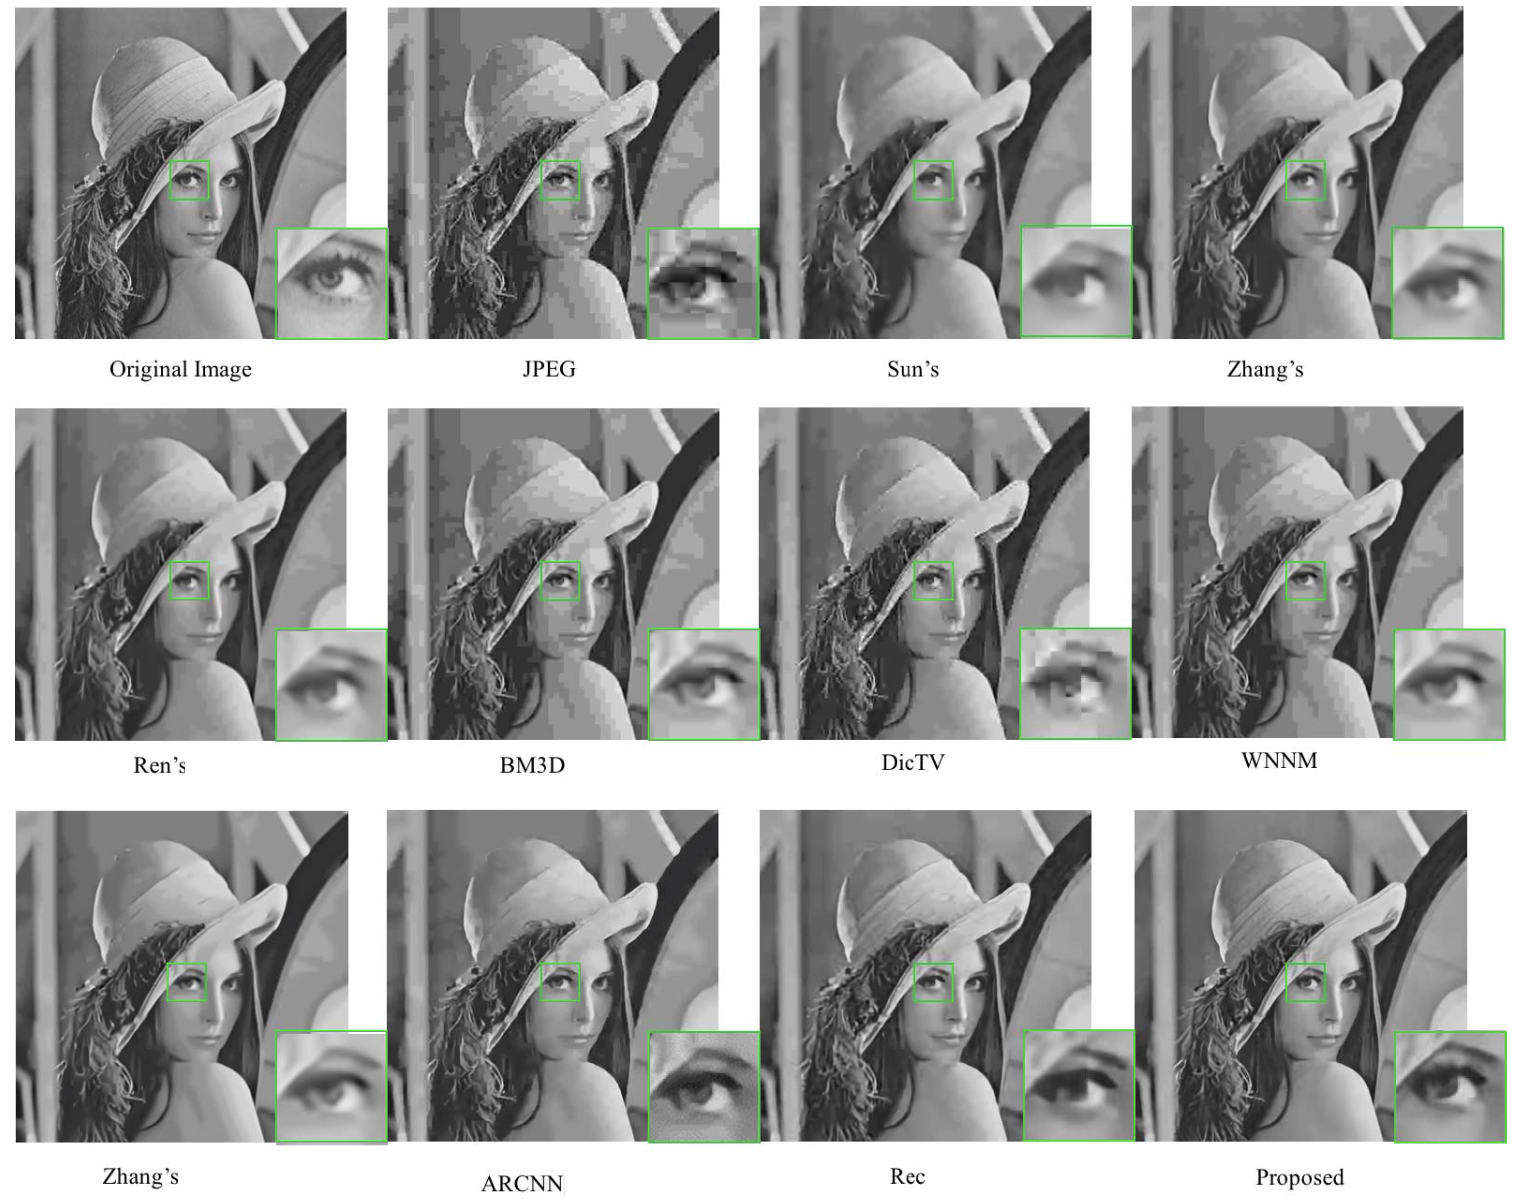
\includegraphics[width = 0.5 \linewidth]{images/paper3/final.png}
        \centering
        \caption{Visual quality comparison of image deblocking ad different QF.}
        \label{fig:final comparison}
    \end{figure}
\end{frame}


\section{Paper 4}
\subsection{\emph{"A Data Set for Camera-Independent Color Constancy"}}

\begin{frame}{INTRODUCTION}
    In computer vision, the output generated by an algorithm depends on the 
    nature of the images set given as input. When the images come from 
    different sources (e.g. different cameras), the behavior of the algorithm is 
    not always the same. For this reason, we try to standardize the input in 
    order to have a more uniform output.
\end{frame}

\begin{frame}{COLOR CONSTANCY DATASETS}
    To produce uniform output, an algorithm must achieve "{\bfseries{color 
    constancy}}" on all input images. In order to calculate this property, there 
    are supervised and unsupervised algorithms. To test the performance of 
    these algorithms, there are already state-of-the-art datasets \footfullcite{0807099130} \footfullcite{0807099132} \footfullcite{0807099120}
    containing indoor and outdoor images, but these have few images inside 
    them.
\end{frame}

\begin{frame}{THE PROPOSED INTEL-TUT DATA SET}
    The purpose of the paper is to present a dataset containing images useful 
    for researching the {\bfseries{camera/scene-independence}} effect of an algorithm.
    To achive this, each scene was captured under five different illumination. 
    In each scene there are images taken from three different cameras, 
    including a mobile one.
    \begin{figure}[htbp]
        \centering
        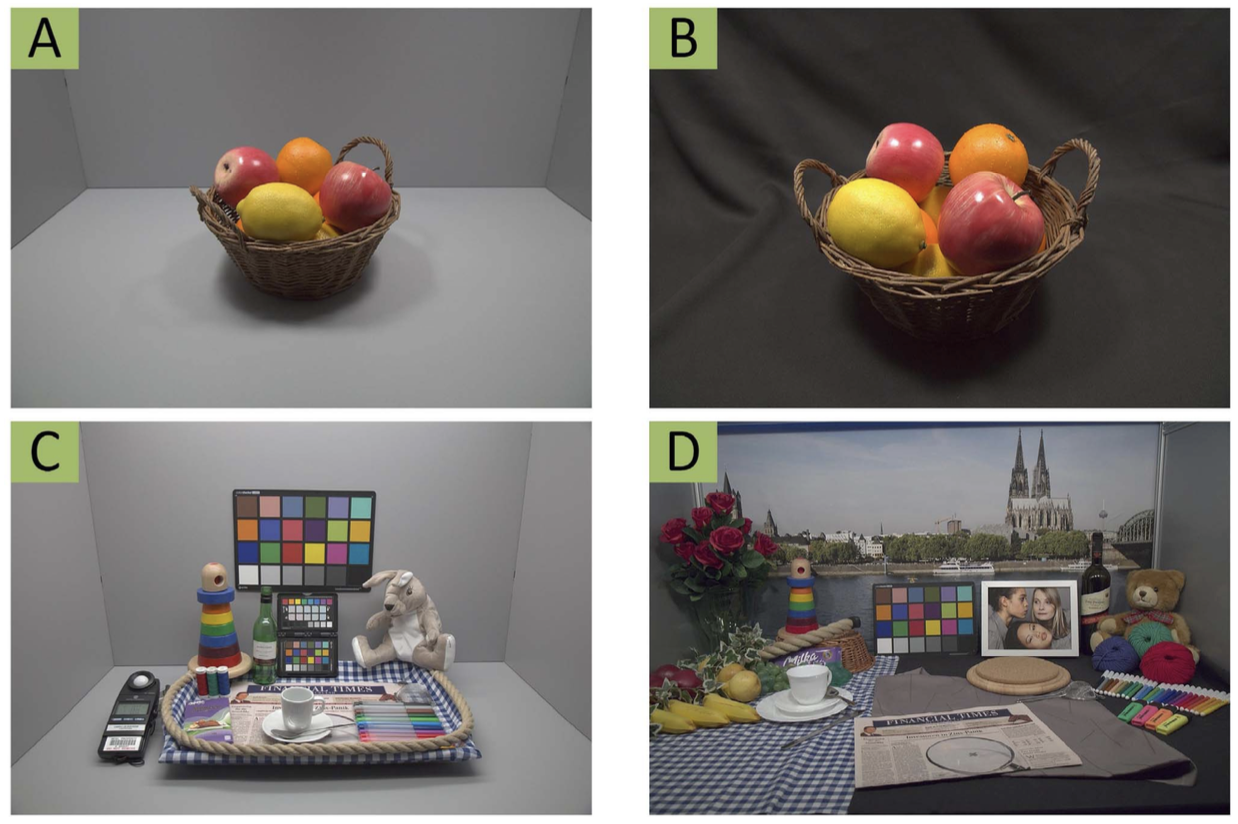
\includegraphics[width = 0.6 \linewidth]{images/paper4/lab.png}
        \centering
        \caption{Lab real scenes}
        \label{fig:Lab}
    \end{figure}
\end{frame}

\begin{frame}{THE PROPOSED INTEL-TUT DATA SET - Chromaticity}
    \begin{block}{Chromatic adaptation - \href{https://en.wikipedia.org/wiki/Color_vision}{\underline{Wikipedia}}}
        \emph{"In color vision, chromatic adaptation refers to color constancy; the 
        ability of the visual system to preserve the appearance of an object under 
        a wide range of light sources."}
    \end{block}
    The only information available on the light source are: the "\emph{Spectral 
    Power Distributions}" (SPD) and the "\emph{Spectral Reflectance}" (SR)
    Thanks to this information, we can obtain the existing chromaticity in the image 
    and compare it with that obtained from the "\emph{Camera Spectral Senstivities}" (CSS).
    \begin{block}{Target}
        The goal is to be able to bring the white point, calculated by each 
        algorithm, closer to the white point of the ground truth, within the same 
        color spectrum (sRGB). To do this, a "\emph{Color Conversion Matrix}" (CMM) 
        is used.
    \end{block}
\end{frame}

\begin{frame}{THE PROPOSED INTEL-TUT DATA SET - Evaluations}
    The performance of supervised and unsupervised methods can be 
    evaluated with 5 of the following strategies:
    \begin{enumerate}
        \item Camera Independence \label{CI}
        \item Camera and Scene Independence
        \item Camera and Scene Independence from Single Camera
        \item Testing the Effect of Color Shading
        \item Testing the Effect of Resolution
    \end{enumerate}
    In each of these strategies, the training set, validation set and testing 
    set contain, in different positions, different images acquired from different 
    cameras.
\end{frame}

\begin{frame}{EXPERIMENTAL RESULTS - Unsupervised methods}
    \begin{block}{Recover Angluar Error}
        Given the chromaticity estimated by the algorithm ($ p^{Est} $) and the 
        effective chromaticity (white point or ground truth) ($ p^E $), the 
        performance of an algorithm can be evaluated based on the result 
        returned by the "\emph{Recovery Angular Error}" (RAE):
        $$ RAE=\cos^{-1}\left(\frac{p^Ep^{Est}}{||p^E||~||p^{Est}||}\right) $$
    \end{block}
    \begin{figure}[htbp]
        \centering
        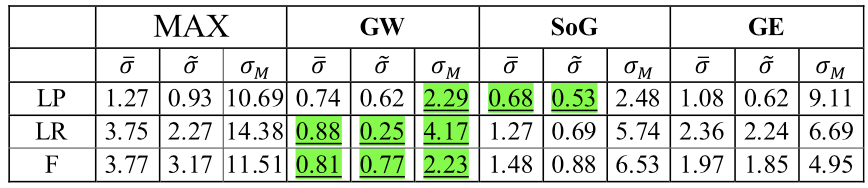
\includegraphics[width = 0.8 \linewidth]{images/paper4/standardHigh.png}
        \centering
        \caption{Mean, Median and Maximum RAE of some algorithms. GW \footfullcite{0807099104} achieves the best performance}
        \label{fig:RAEstandard}
    \end{figure}
\end{frame}
    
\end{document}
